\apendice{Documentación de uso}

\section{Introducción}
En este manual se detallan los requisitos de la aplicación web para poder utilizarla correctamente así como su manual completo de uso de la aplicación dividido en dos partes. La primera de ellas muestra las opciones disponibles para una persona que no tenga cuenta en la aplicación, y la segunda muestra toda la parte que puede utilizar el personal de administración.
\section{Requisitos de uso}
Los requisitos mínimos de la aplicación web son los siguientes:
\begin{itemize}
    \item Conexión a internet
    \item Un navegador web para entrar a la siguiente URL: \href{https://prehistoriaenigualdad.netlify.app/}{Prehistoria en igualdad}
\end{itemize}
\section{Instalación}
En este caso no se necesita realizar ningún tipo de instalación, ya que en todos los dispositivos ya existe por defecto un navegador con el que poder entrar a la aplicación web.
\section{Manual del usuario/a sin cuenta}
En este apartado se recogen todas las acciones que puede realizar un usuario que no se encuentre registrado en la aplicación web.

\subsection{Consultar en el catálogo un libro}
Una de las funciones principales de esta aplicación es mostrar información a docentes y familias acerca de los libros analizados. Existen dos opciones para realizar esta operación.

\begin{enumerate}
    \item Desde el inicio.
    \begin{itemize}
        \item Rellenar el campo de búsqueda con un ISBN o con un Título.
        \item Automáticamente se redirige al catálogo con la búsqueda completada mostrando el libro deseado al hacer click en el botón de buscar.
    \end{itemize}
    \item Realizando la búsqueda desde el catálogo.
    \begin{itemize}
        \item Hacer click en el menú superior en el botón catálogo
        \item Rellenar el campo de búsqueda con ISBN o Título.
        \item Hacer click en la lupa para realizar la búsqueda.
        \item Se mostrarán los libros que coincidan con los parámetros de la búsqueda
    \end{itemize}
\end{enumerate}


\begin{figure}[h]
    \centering
    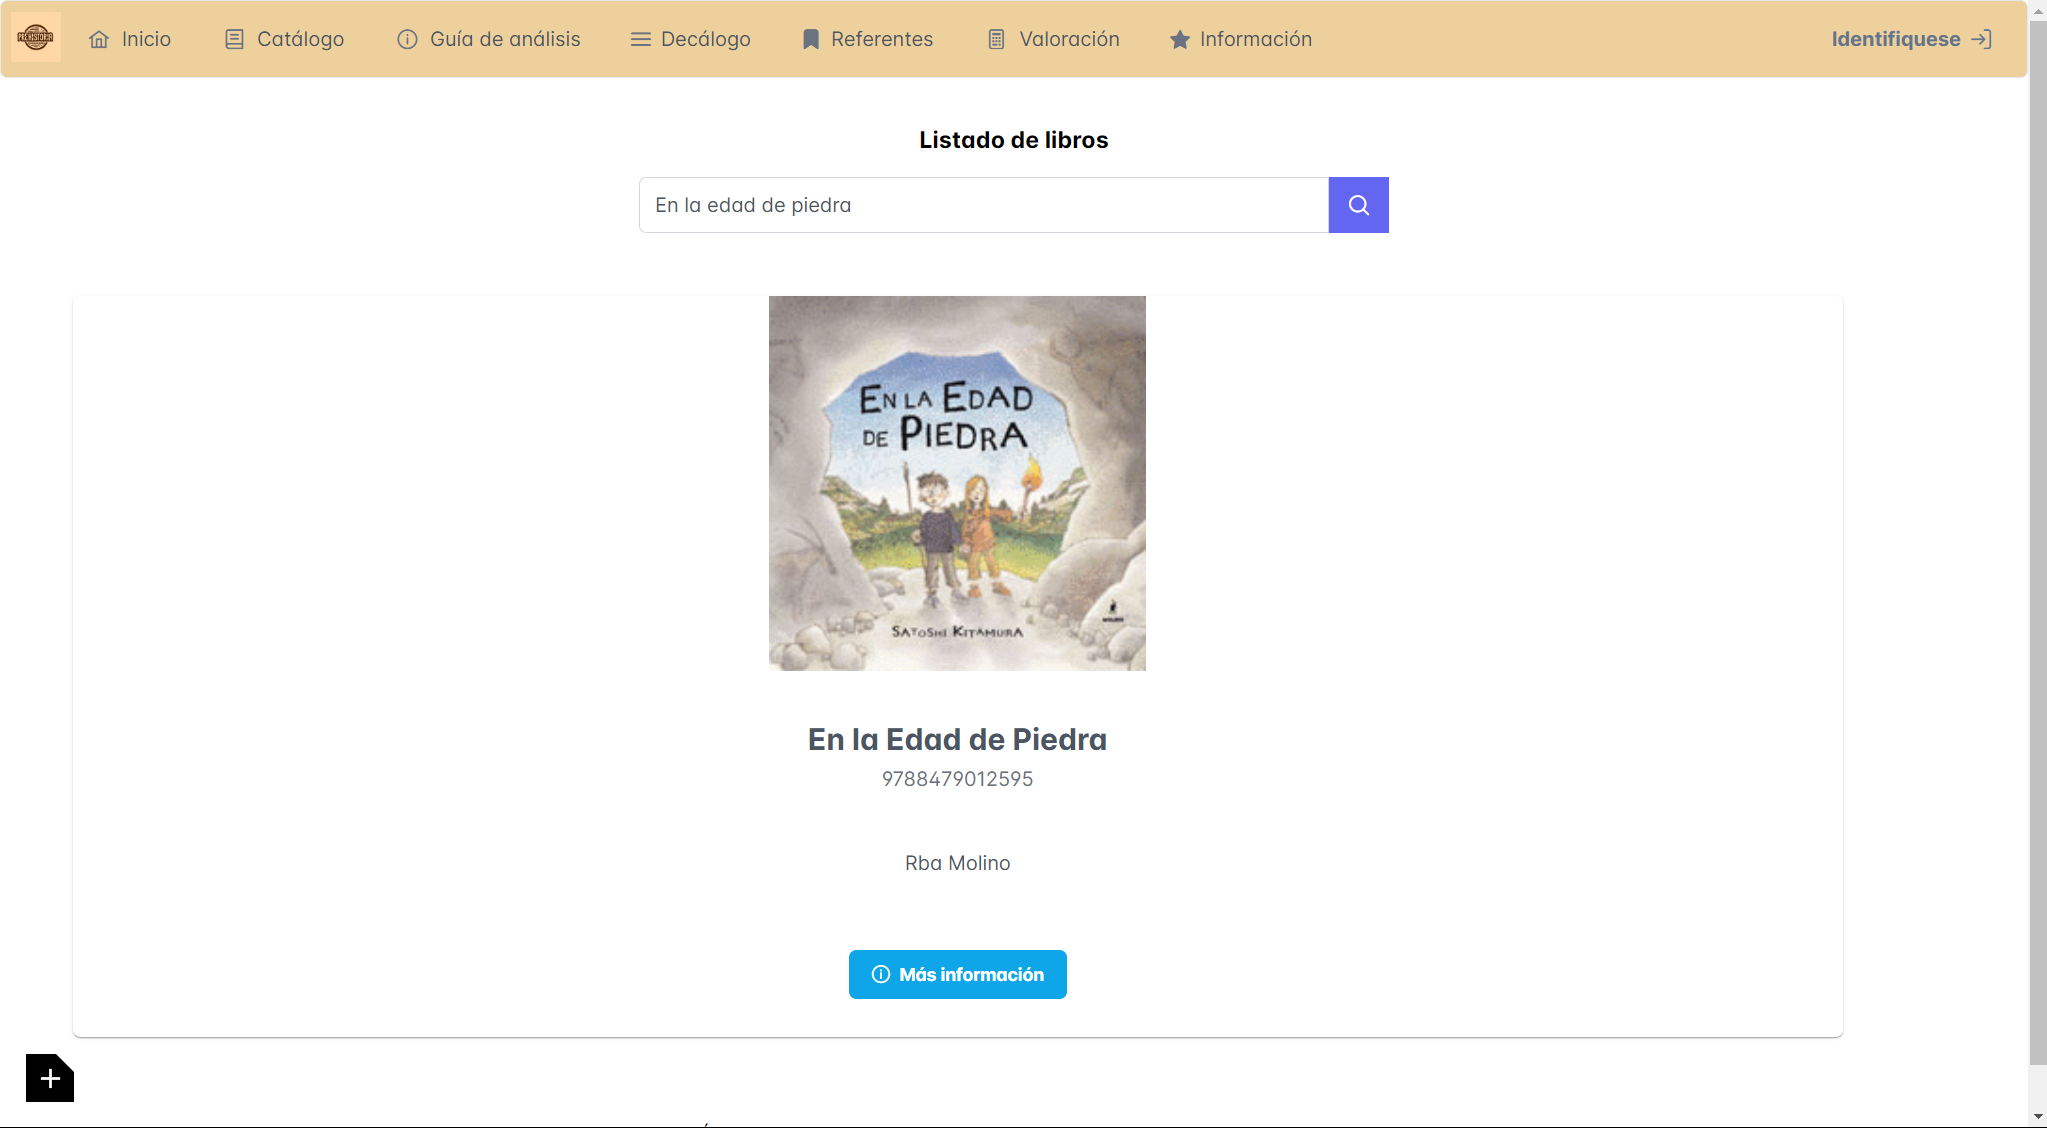
\includegraphics[width=1\linewidth]{Imagenes/ManualBusquedaLibro.png}
    \caption{Búsqueda de libro en catálogo}
    \label{Búsuqeda de libro en catálogo}
\end{figure}
\FloatBarrier

\subsection{Consultar la información de un libro}
Si un usuario/a conoce un libro sobre el que quiere consultar toda su información, se han de realizar los siguientes pasos. 

\begin{itemize}
    \item Buscar un libro desde inicio o desde el catálogo.
    \item Seleccionar el botón de más información del libro deseado.
    \item Hacer click en el botón de más información correspondiente a ese libro
\end{itemize}
Las acciones que se pueden realizar dentro de este apartado son los siguientes:
\begin{enumerate}
    \item Si se hace click en el símbolo de información, la web cargará la pestaña de la guía de análisis.
    \item El apartado de la ubicación del estudio, si contiene información, es un hipervínculo que lleva a la dirección del estudio de ese libro
\end{enumerate}
\begin{figure}[h]
    \centering
    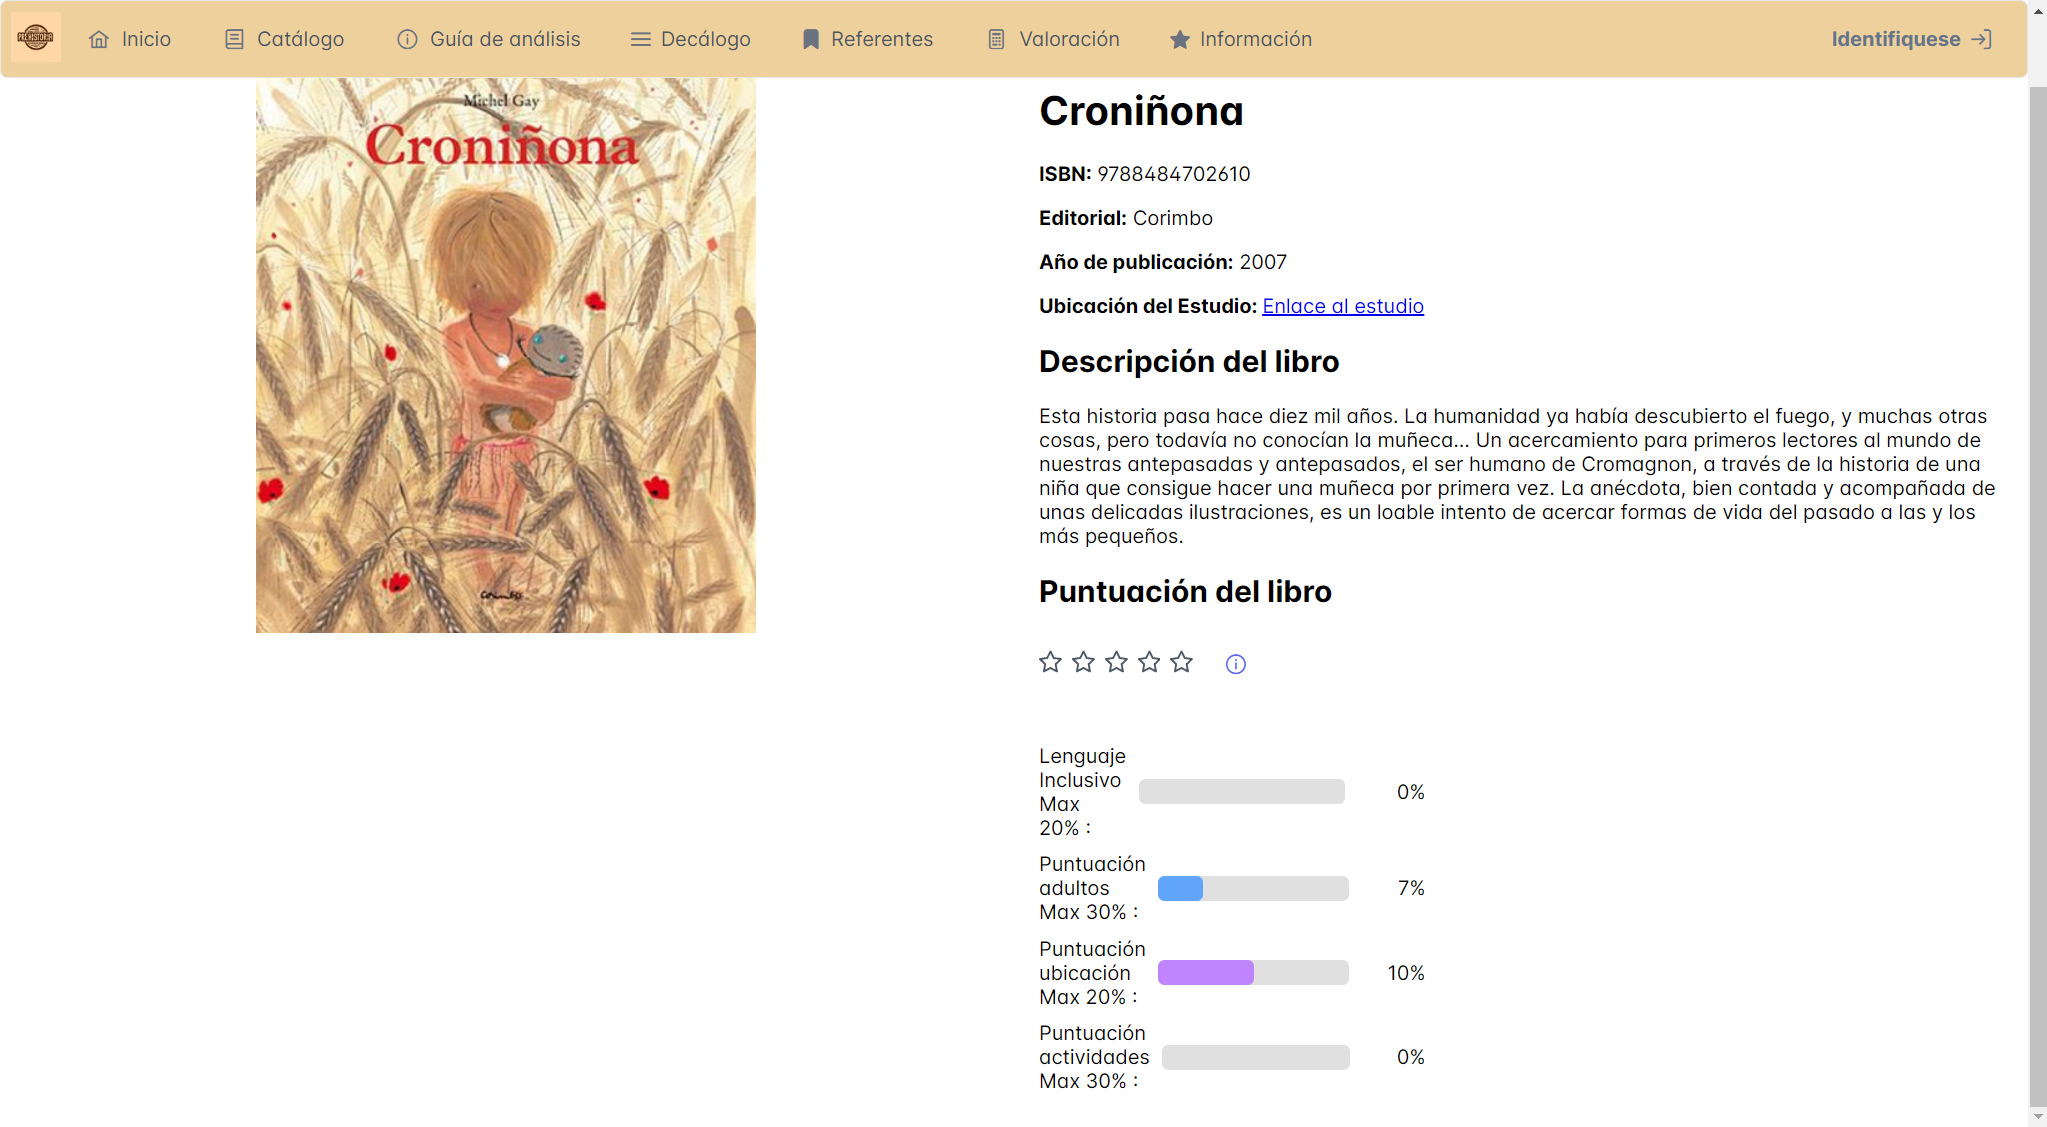
\includegraphics[width=1\linewidth]{Imagenes/ManualMasInfo.png}
    \caption{Más información de un libro}
    \label{Más información de un libro}
\end{figure}
\FloatBarrier

\subsection{Sugerir un libro}
Prehistoria en Igualdad permite a los usuarios realizar recomendaciones al personal de administración para que agreguen nuevos libros al catálogo que puedan ser interesantes de cara a los objetivos de esta aplicación.

Para realizar una sugerencia de un libro:
\begin{itemize}
    \item Entrar en el apartado de catálogo
    \item Pulsar el botón con el icono de un '+' situado abajo a la izquierda.
    \item Rellenar el formulario con los campos solicitados y enviar.
\end{itemize}
\begin{figure}[h]
    \centering
    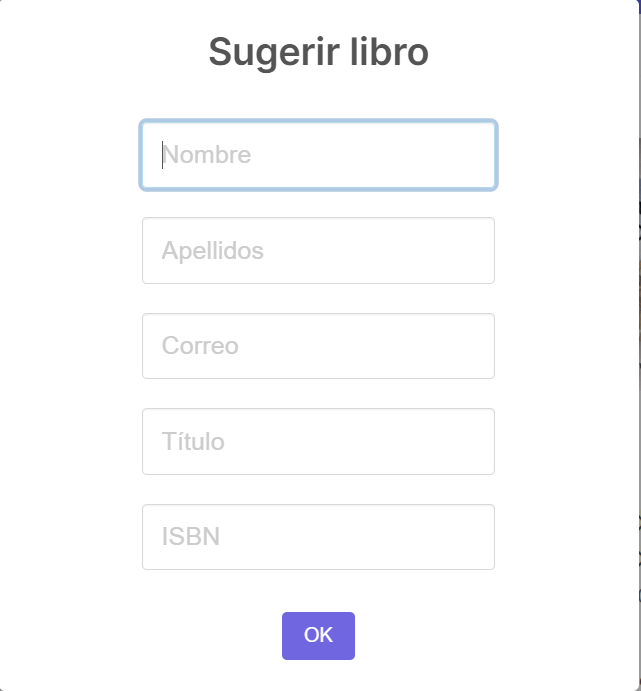
\includegraphics[width=0.6\linewidth]{Imagenes/ManualSugerencia.png}
    \caption{Formulario de sugerencia de libro}
    \label{Formulario de sugerencia de libro}
\end{figure}
\FloatBarrier

\subsection{Realizar una valoración}
Otra de las partes fundamentales de esta aplicación web es la posibilidad que tienen los docentes y familias de realizar sus propias valoraciones de los libros que deseen. Los pasos para realizarla son los siguientes:

\begin{itemize}
    \item Desde el menú acceder a la pestaña de valoración
    \item Rellenar los campos existentes utilizando como base la guía de análisis
    \item Pulsar el botón de calcular.
    \item Una vez se realiza el cálculo, aparecerá una modal con el resultado del cálculo y 3 opciones, navegar a la guía de análisis, no guardar la estimación, o guardarla
    \begin{figure}[h]
        \centering
        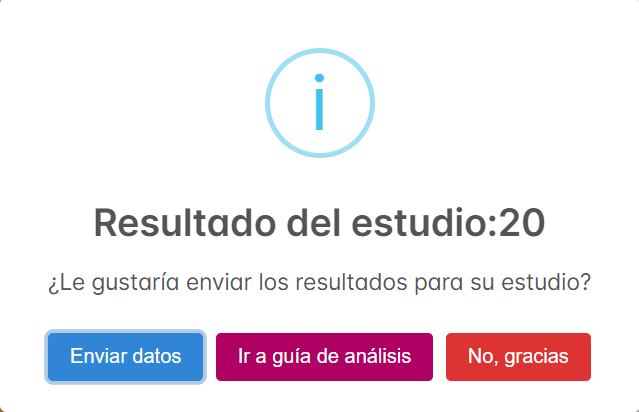
\includegraphics[width=0.6\linewidth]{Imagenes/ManualResultadoValoracion.png}
        \caption{Resultado de valoración}
        \label{Resultado de valoración}
    \end{figure}
    \FloatBarrier
    
    \item En el caso de que se guarde la estimación, aparecerá un formulario para rellenar con los datos personales (opcionales) por si es necesario ponerse en contacto con la persona que la ha realizado.
    \begin{figure}[h]
        \centering
        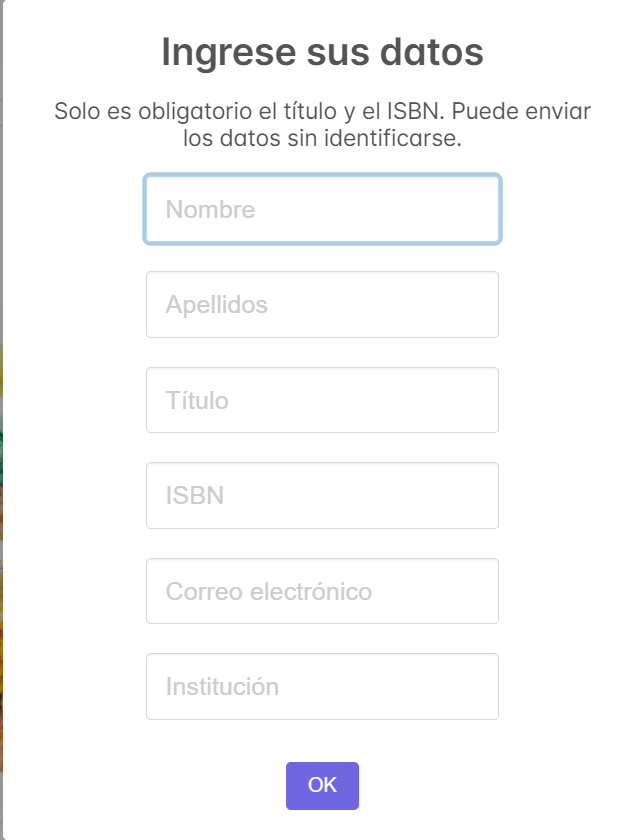
\includegraphics[width=0.5\linewidth]{Imagenes/ManualGuardarValoracion.png}
        \caption{Guardar valoración}
        \label{Guardar valoración}
    \end{figure}
\end{itemize}
\FloatBarrier

\section{Manual del usuario/a con cuenta y permisos de administración}
Antes de continuar con los siguientes apartados, hay que tener en cuenta que todas las operaciones que se realizan por un usuario sin cuenta las puede realizar un usuario con cuenta, por lo que el manual de la sección anterior es válido también para usuarios y usuarias autenticadas. Además de esta aplicación web, está disponible una cuenta de correo electrónico donde se reciben todas las sugerencias realizadas por los usuarios.

\subsection{Iniciar sesión}
Para poder acceder a la zona de administración para realizar todas las operaciones de gestión, han de seguirse los siguientes pasos:
\begin{itemize}
    \item Se selecciona en el menú superior el botón Identifíquese.
    \item Se rellena el campo de usuario y de contraseña para iniciar sesión.
    \begin{figure}[h]
        \centering
        \includegraphics[width=0.6\linewidth]{Imagenes/ManualInicioSesión.png}
        \caption{Manual de Inicio de sesión}
        \label{Manual de Inicio de sesión}
    \end{figure}
    \FloatBarrier
    \item Si se ha iniciado sesión correctamente se redirigirá al catálogo, y en el menú superior, donde se encontraba el botón de identifíquese aparecerá el nombre del usuario y un desplegable que permite acceder al panel de administración y cerrar sesión.
\end{itemize}
\begin{figure}[h]
        \centering
        
\includegraphics[width=0.4\linewidth]{Imagenes/MenuNombreAdmin.png}
        \caption{Cambio de botón Inicio de sesión}
        \label{Cambio de botón Inicio de sesión}
    \end{figure}
    \FloatBarrier

\subsection{Consultar estadísticas de la aplicación web}
Actualmente todo el equipo de administración tiene a su disposición unas métricas mensuales que muestran distintos elementos informativos para consultar de manera gráfica el estado de la aplicación.
A este apartado se accede desde el botón del panel de administrador.
\begin{figure}
    \centering
    \includegraphics[width=1\linewidth]{Imagenes/ManualEstadísticas.png}
    \caption{Estadísticas de administración}
    \label{Estadísticas de administración}
\end{figure}

La información que muestran estas estadísticas es la siguiente:
\begin{itemize}
    \item El primer gráfico muestra el número de visitas totales que se ha tenido este mes entre todos los libros y las visitas del libro más popular.
    \item En el segundo gráfico se puede observar el número de usuarios/as registradas en la aplicación.
    \item El tercer gráfico muestra con gráficos de líneas el número de libros existentes, sugerencias enviadas y estimaciones realizadas cada mes.
    \item El cuarto elemento es una tarjeta donde se indica cuál ha sido el libro más popular.
    \items
\end{itemize}
Cabe destacar que existe la opción de filtrar los datos para acotar los datos en una franja temporal determinada. Por motivos de diseño el máximo de meses a mostrar son 12.

\subsection{Gestión de personas usuarias}
Este apartado es el encargado de dar todas las herramientas que necesite el equipo de administración para tener un control total de quién puede formar parte o no de ese equipo.

Los pasos para realizar una operación en este apartado son los siguientes:
\begin{itemize}
    \item Acceder al panel de administración desde el menú superior.
    \item Desplegar el menú lateral disponible en el menú de administración y seleccionar 'gestión de personas'.
    \item La aplicación muestra las cuentas existentes.
    \item Si se desea crear un nuevo usuario/a:
    \begin{enumerate}
        \item Hacer click en el botón de nuevo usuario.
        \item Rellenar el formulario que se ha desplegado con un nombre, correo y el rol deseado. Si no se selecciona rol, se establece uno predefinido.
        \item Si se ha creado correctamente, aparecerá una modal indicando la contraseña temporal de esa cuenta.
    \end{enumerate}
    \item Si se desea modificar un usuario/a  existente:
    \begin{enumerate}
        \item Hacer click en el lápiz correspondiente a ese usuario/a.
        \item Modificar el formulario que se ha desplegado autocompletado con el nombre, correo y el rol asignado.
        \item Si se ha modificado correctamente, aparecerá una modal indicando éxito en la operación.
    \end{enumerate}
    \item Si se desea eliminar un usuario/a:
    \begin{enumerate}
        \item Hacer click en la papelera correspondiente a ese usuario/a.
        \item Confirmar en la modal la operación por seguridad.
        \item Si se ha eliminado correctamente, aparecerá una modal indicando éxito en la operación.
    \end{enumerate}
\end{itemize}
\begin{figure}[h]
    \centering
    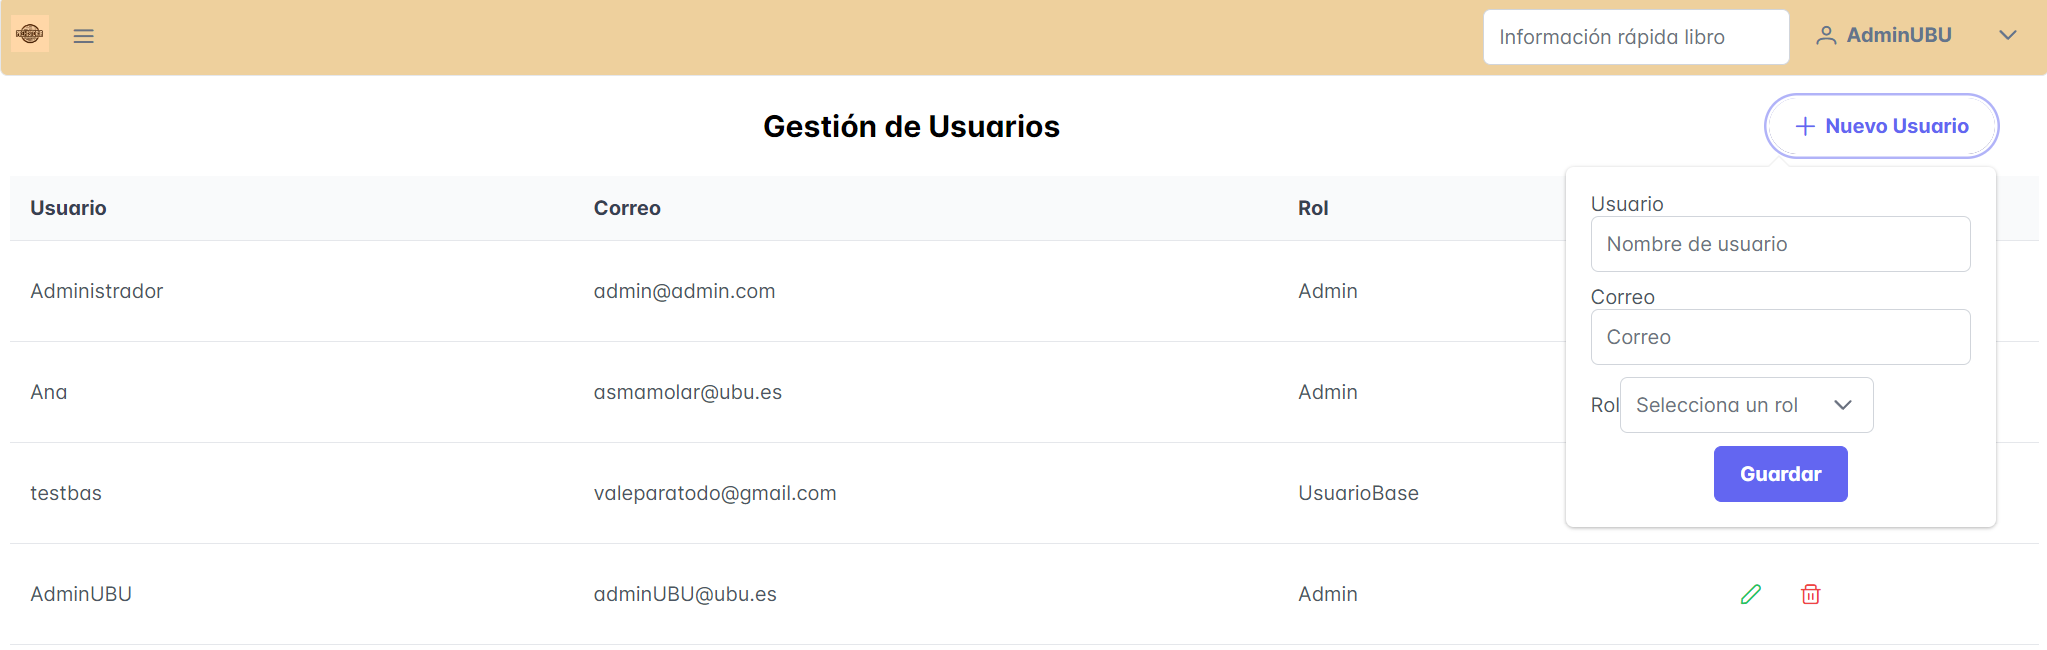
\includegraphics[width=1\linewidth]{Imagenes/ManualUsuarios.png}
    \caption{Operaciones en gestión de usuarios/as}
    \label{Operaciones en gestión de usuarios/as}
\end{figure}
\FloatBarrier

\subsection{Gestión de roles}
Para poder gestionar la autorización de acceso a ciertas funcionalidades de la aplicación, se ha diseñado un sistema de permisos utilizando roles que limitan estas acciones de manera dinámica.

\begin{itemize}
    \item Acceder al panel de administración desde el menú superior.
    \item Desplegar el menú lateral disponible en el menú de administración y seleccionar 'gestión de roles'.
    \item La aplicación muestra los roles existentes.
    \item Si se desea crear un nuevo rol:
    \begin{enumerate}
        \item Hacer click en el botón de nuevo usuario.
        \item Introducir el nombre deseado.
        \item Si se ha creado correctamente, aparecerá una modal el éxito de la operación.
    \end{enumerate}
    \item Si se desea modificar un rol existente:
    \begin{enumerate}
        \item Hacer click en el lápiz correspondiente a ese rol.
        \item Introducir el nuevo nombre de rol deseado.
        \item Si se ha modificado correctamente, aparecerá una modal indicando éxito en la operación.
    \end{enumerate}
    \item Si se desea eliminar un rol:
    \begin{enumerate}
        \item Hacer click en la papelera correspondiente a ese rol.
        \item Confirmar en la modal la operación por seguridad.
        \item Si se ha eliminado correctamente, aparecerá una modal indicando éxito en la operación.
    \end{enumerate}

    \begin{figure}[h]
        \centering
        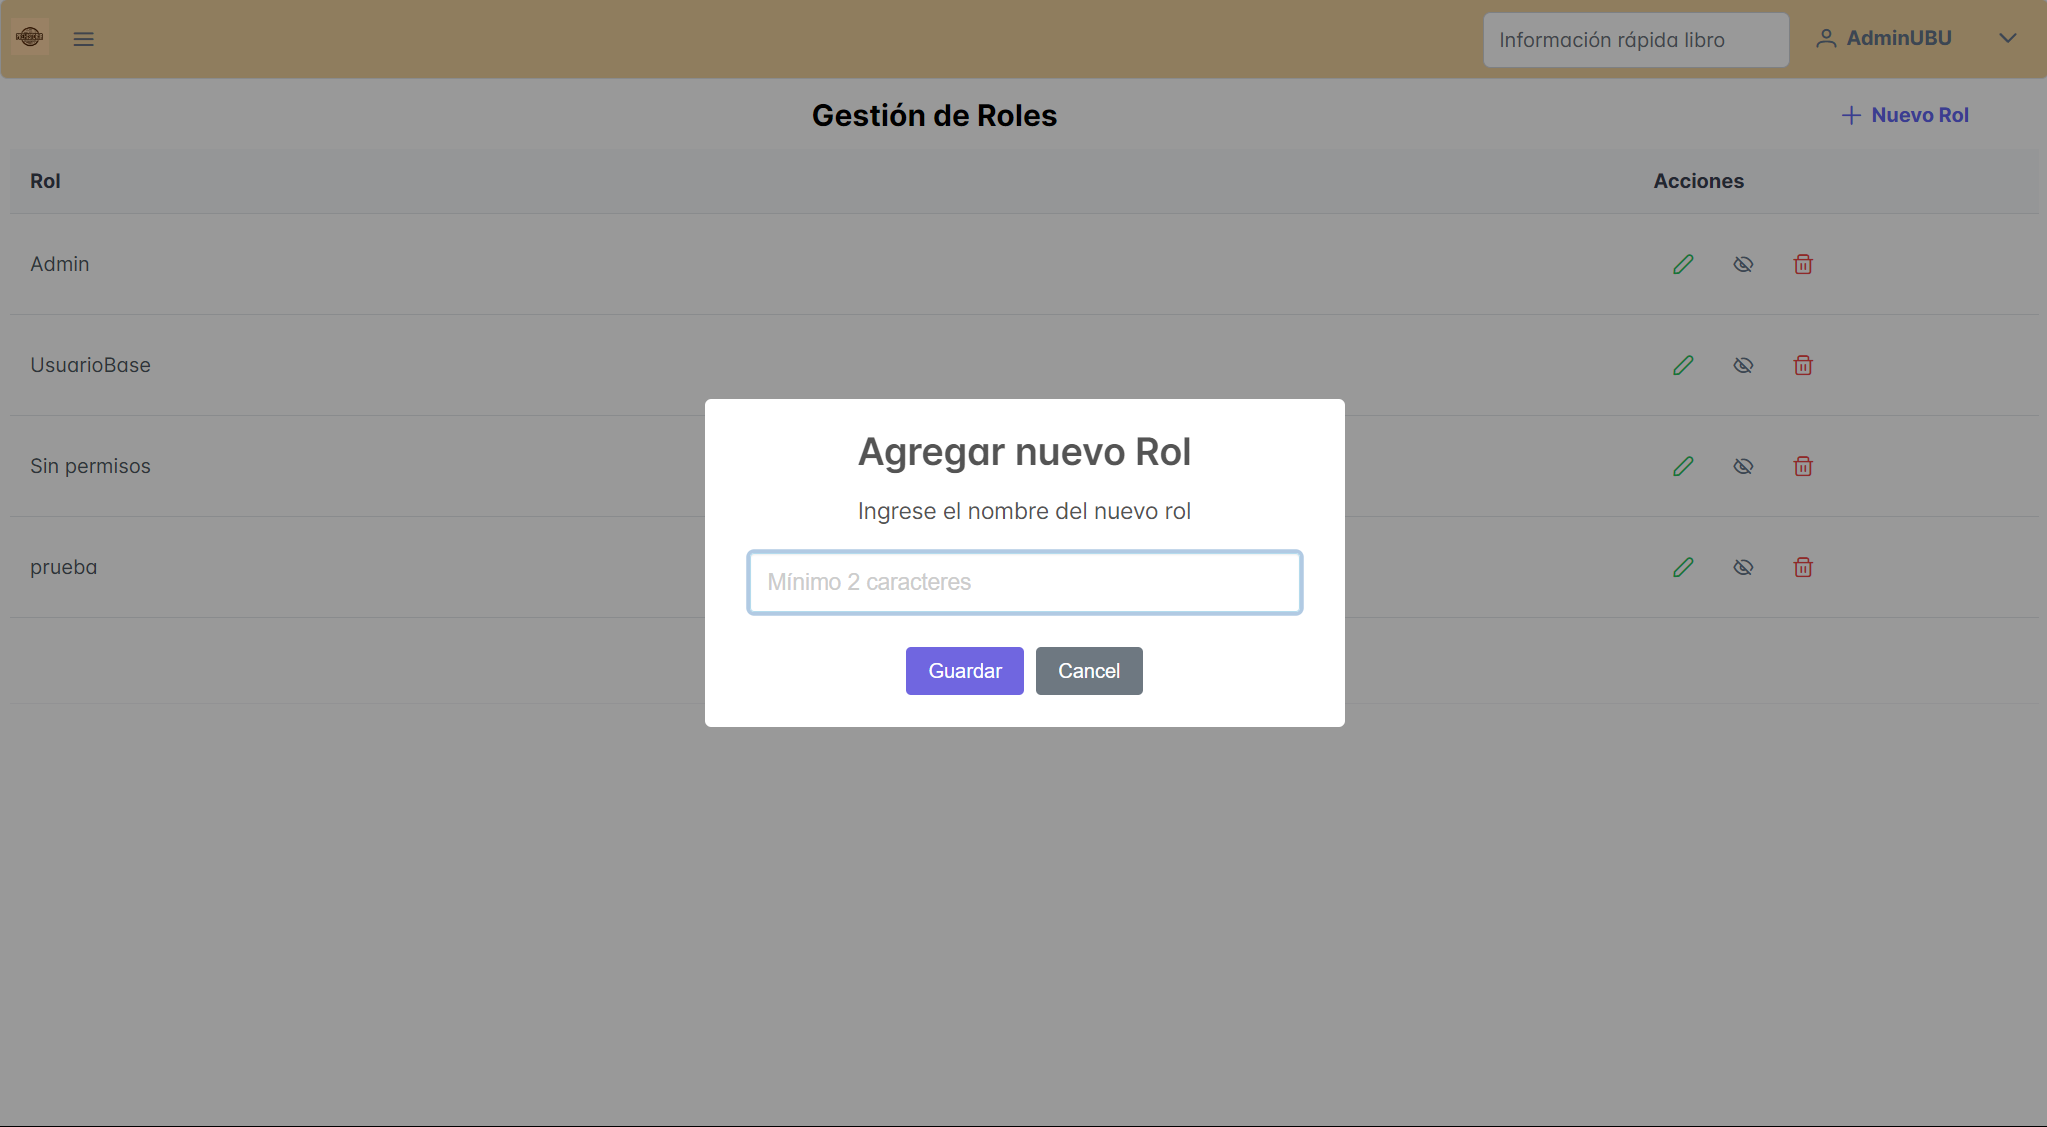
\includegraphics[width=1\linewidth]{Imagenes/ManualRol.png}
        \caption{Operación agregar rol en gestión de roles}
        \label{Operación agregar rol en gestión de roles}
    \end{figure}
    \FloatBarrier

    \item Si se desean gestionar los permisos correspondientes a un rol, ha de seleccionarse el icono del ojo en el rol deseado.
    \item Activar y desactivar los permisos asociados a ese rol y guardar cambios.
\end{itemize}
\begin{figure}[h]
    \centering
    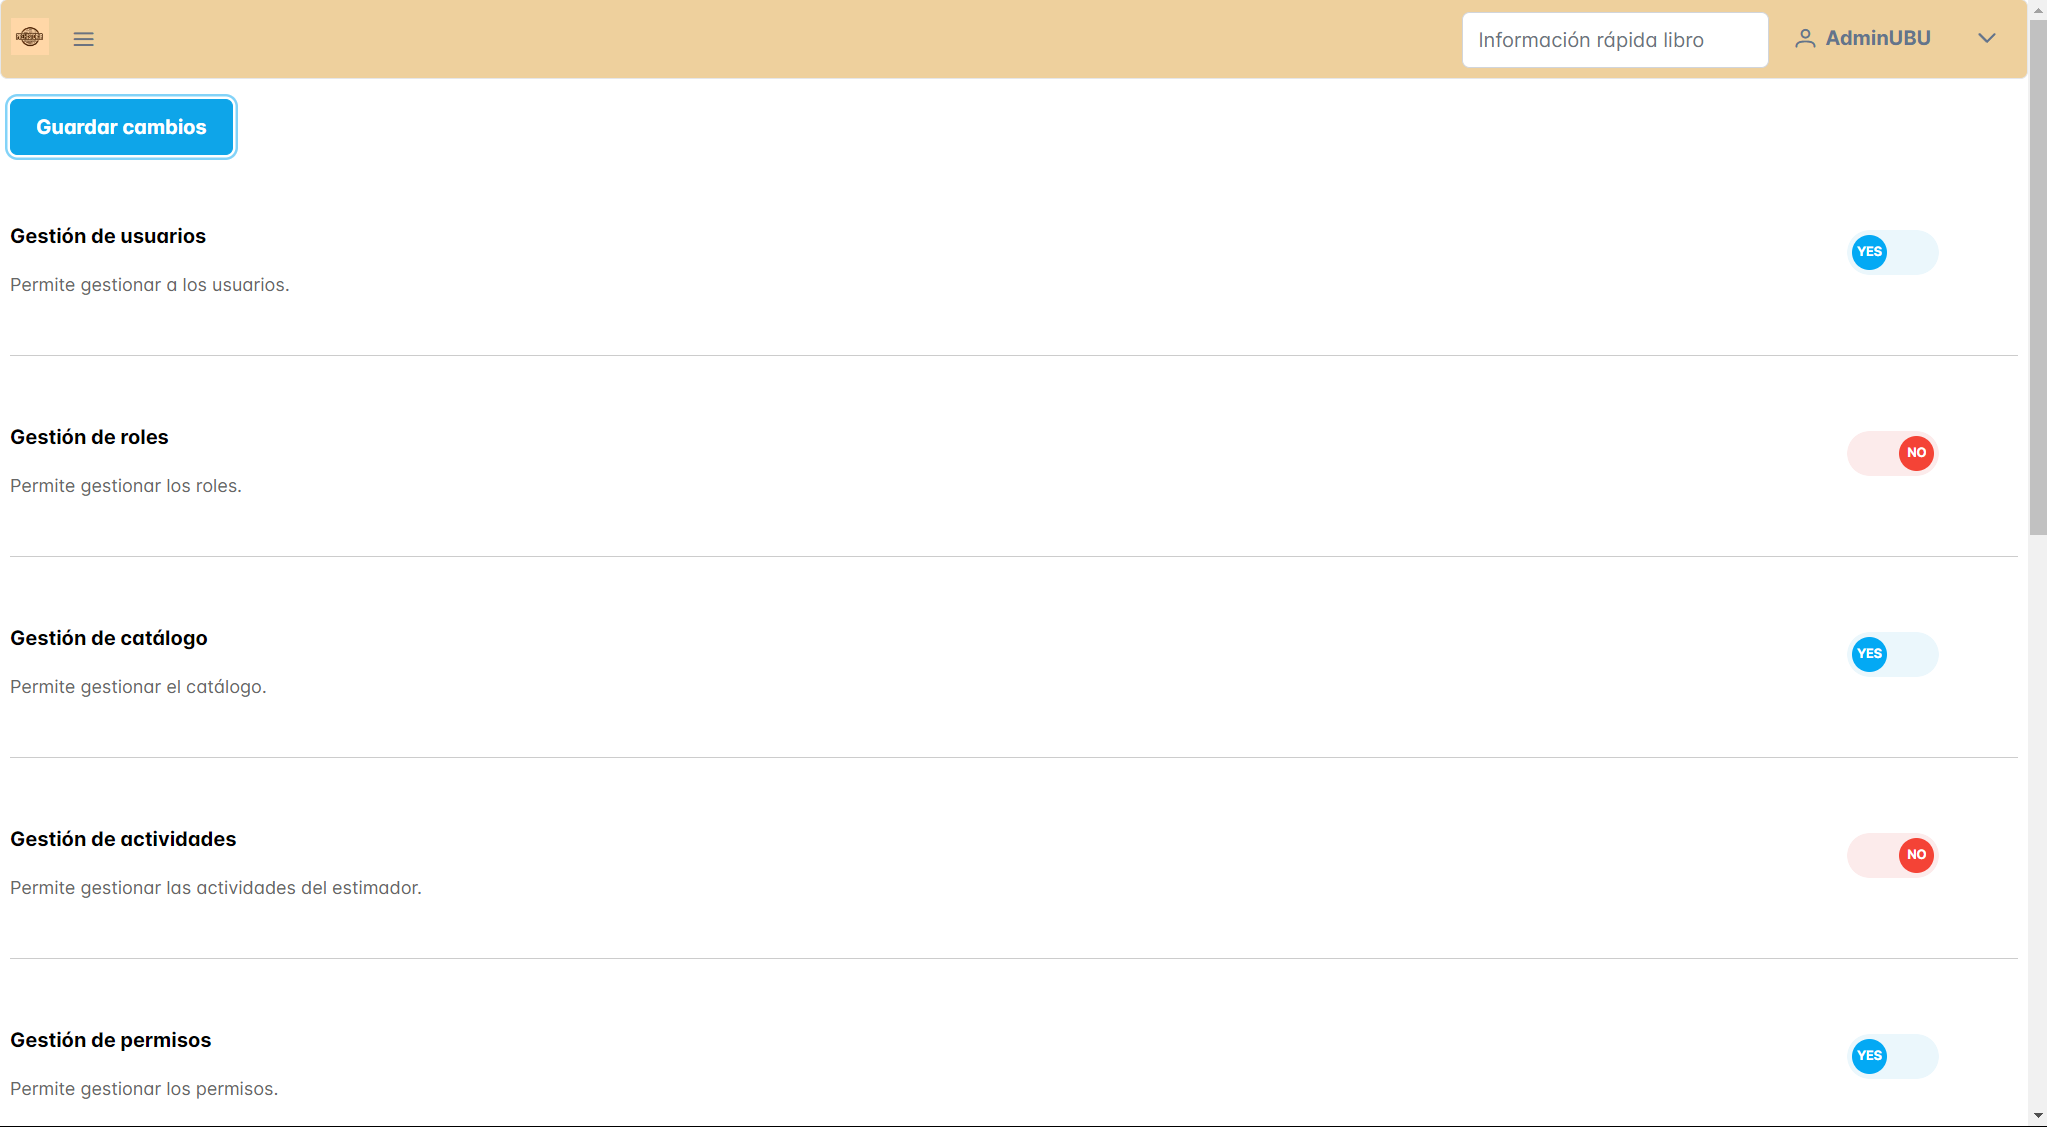
\includegraphics[width=1\linewidth]{Imagenes/ManualPermisos.png}
    \caption{Permisos de un rol}
    \label{Permisos de un rol}
\end{figure}
\FloatBarrier


\subsection{Gestión de colaboradores}
Los colaboradores de esta aplicación web son todos aquellos usuarios/as que han realizado una valoración de un libro la cuál aporte datos objetivos y se considere que ese libro se puede incluir en el catálogo. Para gestionar los colaboradores existentes se han de realizar los siguientes pasos.
\begin{itemize}
    \item Acceder al panel de administración desde el menú superior.
    \item Desplegar el menú lateral ubicado en el menú de administración y seleccionamos 'gestión de colaboradores'.
    \item La aplicación muestra los colaboradores existentes.
    \item Si se desea agregar un nuevo colaborador:
    \begin{enumerate}
        \item Hacer click en el botón Nuevo colaborador.
        \item Rellenar el desplegable con los campos pedidos.
        \item Guardar los cambios.
    \end{enumerate}
    \item Si se desea editar un colaborador:
    \begin{enumerate}
        \item Hacer click en el lápiz correspondiente al colaborador.
        \item Modificar el desplegable con los campos deseados.
        \item Guardar los cambios.
    \end{enumerate}
    \item Si se desea eliminar un colaborador:
    \begin{enumerate}
        \item Hacer click en la papelera correspondiente.
        \item Confirmar en la modal la operación.
    \end{enumerate}
\end{itemize}
\begin{figure}[h]
    \centering
    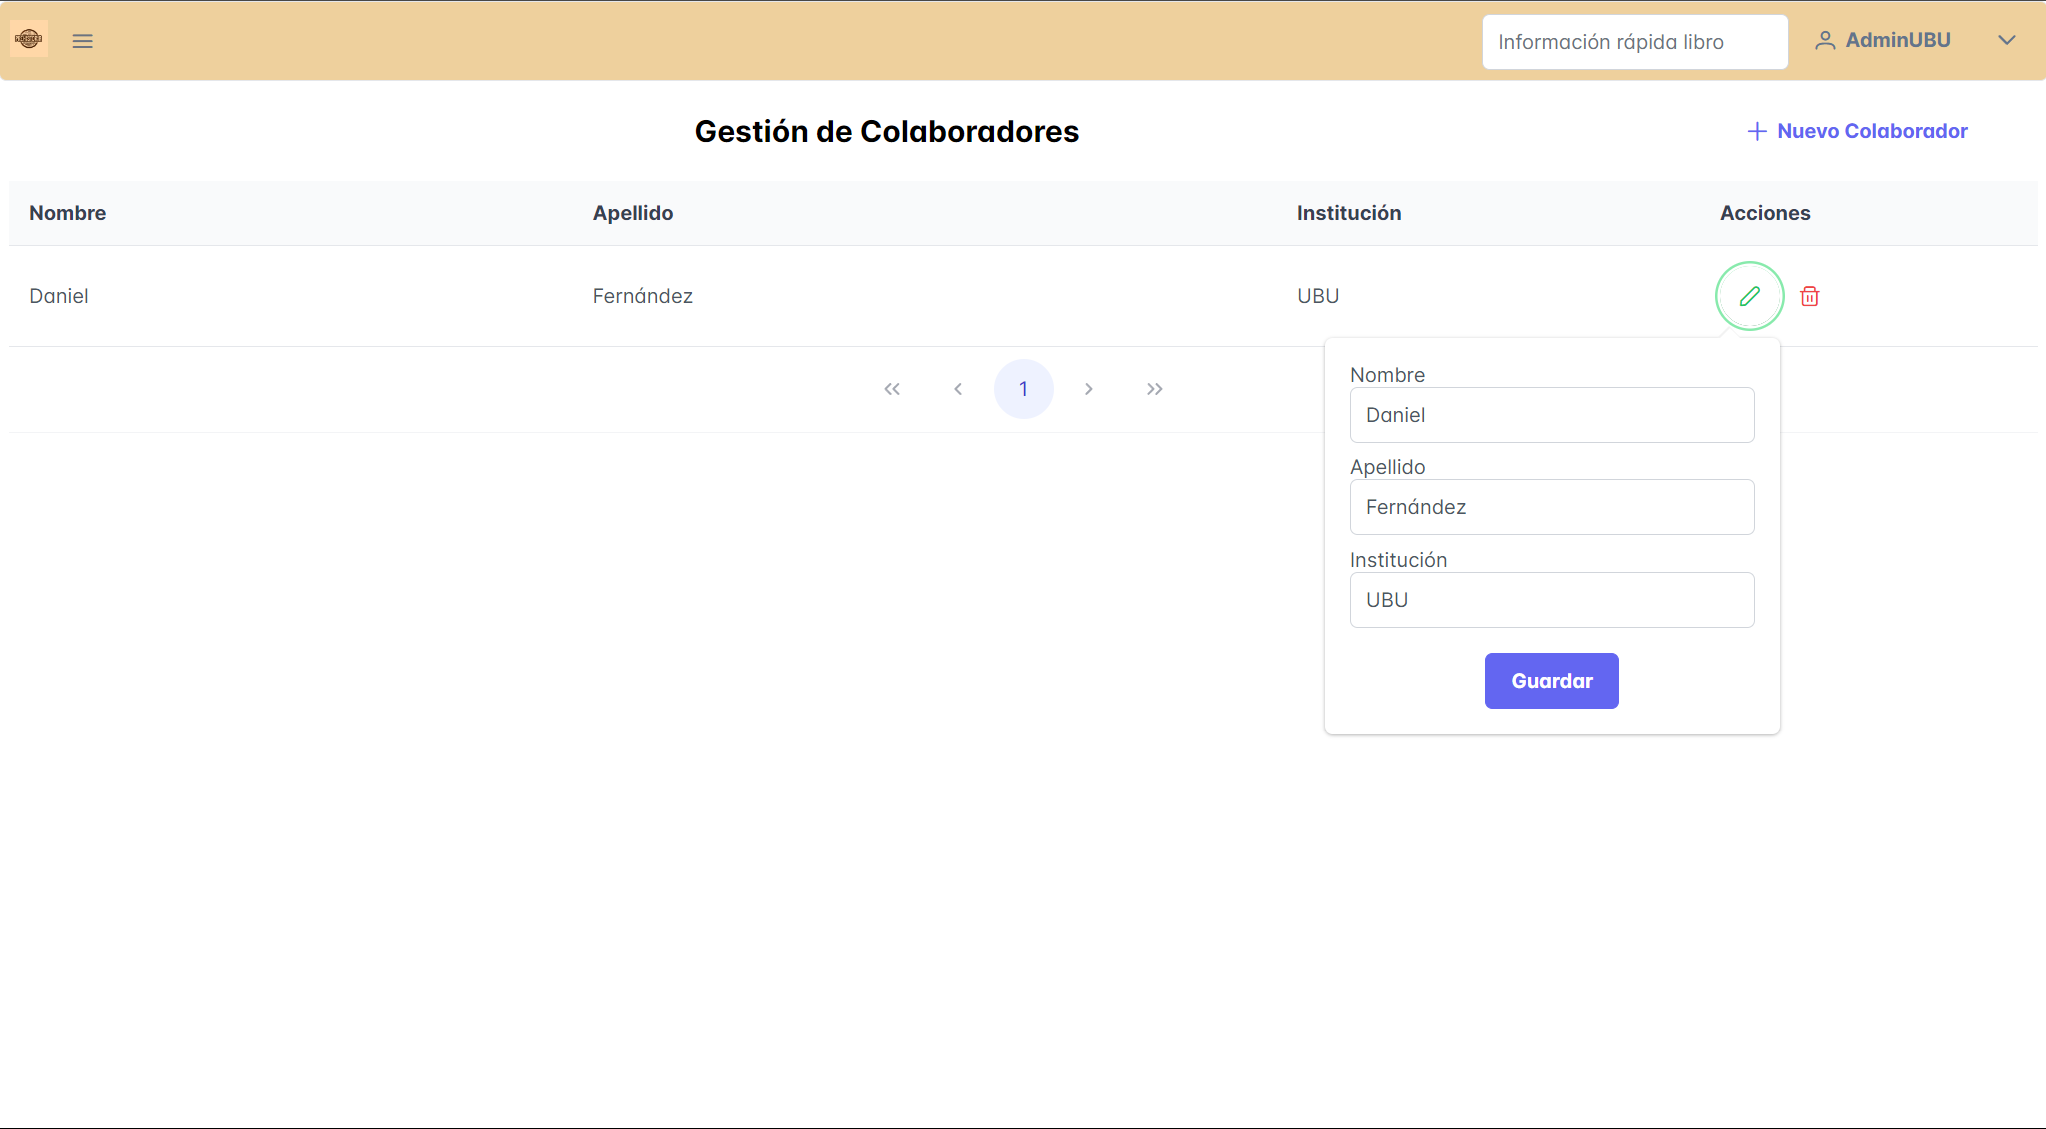
\includegraphics[width=1\linewidth]{Imagenes/ManualColaboraciones.png}
    \caption{Panel de gestión de colaboradores}
    \label{Panel de gestión de colaboradores}
\end{figure}
\FloatBarrier

\subsection{Agregar un nuevo libro}
Una de las piezas fundamentales de esta aplicación es el catálogo y todos sus elementos de gestión que lo rodean. Este apartado va dirigido a explicar las 2 maneras existentes en la aplicación de añadir libros en el catálogo.

\subsubsection{Agregar un libro manualmente}
La forma de agregar un libro manualmente es agregando todos los campos de la información del libro a mano, por lo que se tiene que buscar toda la información.
Los pasos son los siguientes:
\begin{itemize}
    \item Acceder al panel de administración desde el menú superior.
    \item Desplegar el menú lateral ubicado en el menú de administración y seleccionamos la opción 'agregar libro'.
    \item La aplicación muestra un formulario completo con todos los datos que han de incluirse para que se reflejen en el catálogo.
    \item Se rellenan todos los campos (Si ubicación del estudio se queda vacío el programa lo va a sustituir por no disponible).
    \item Si se guarda correctamente la aplicación mostrará una modal indicándolo
\end{itemize}
\begin{figure}
    \centering
    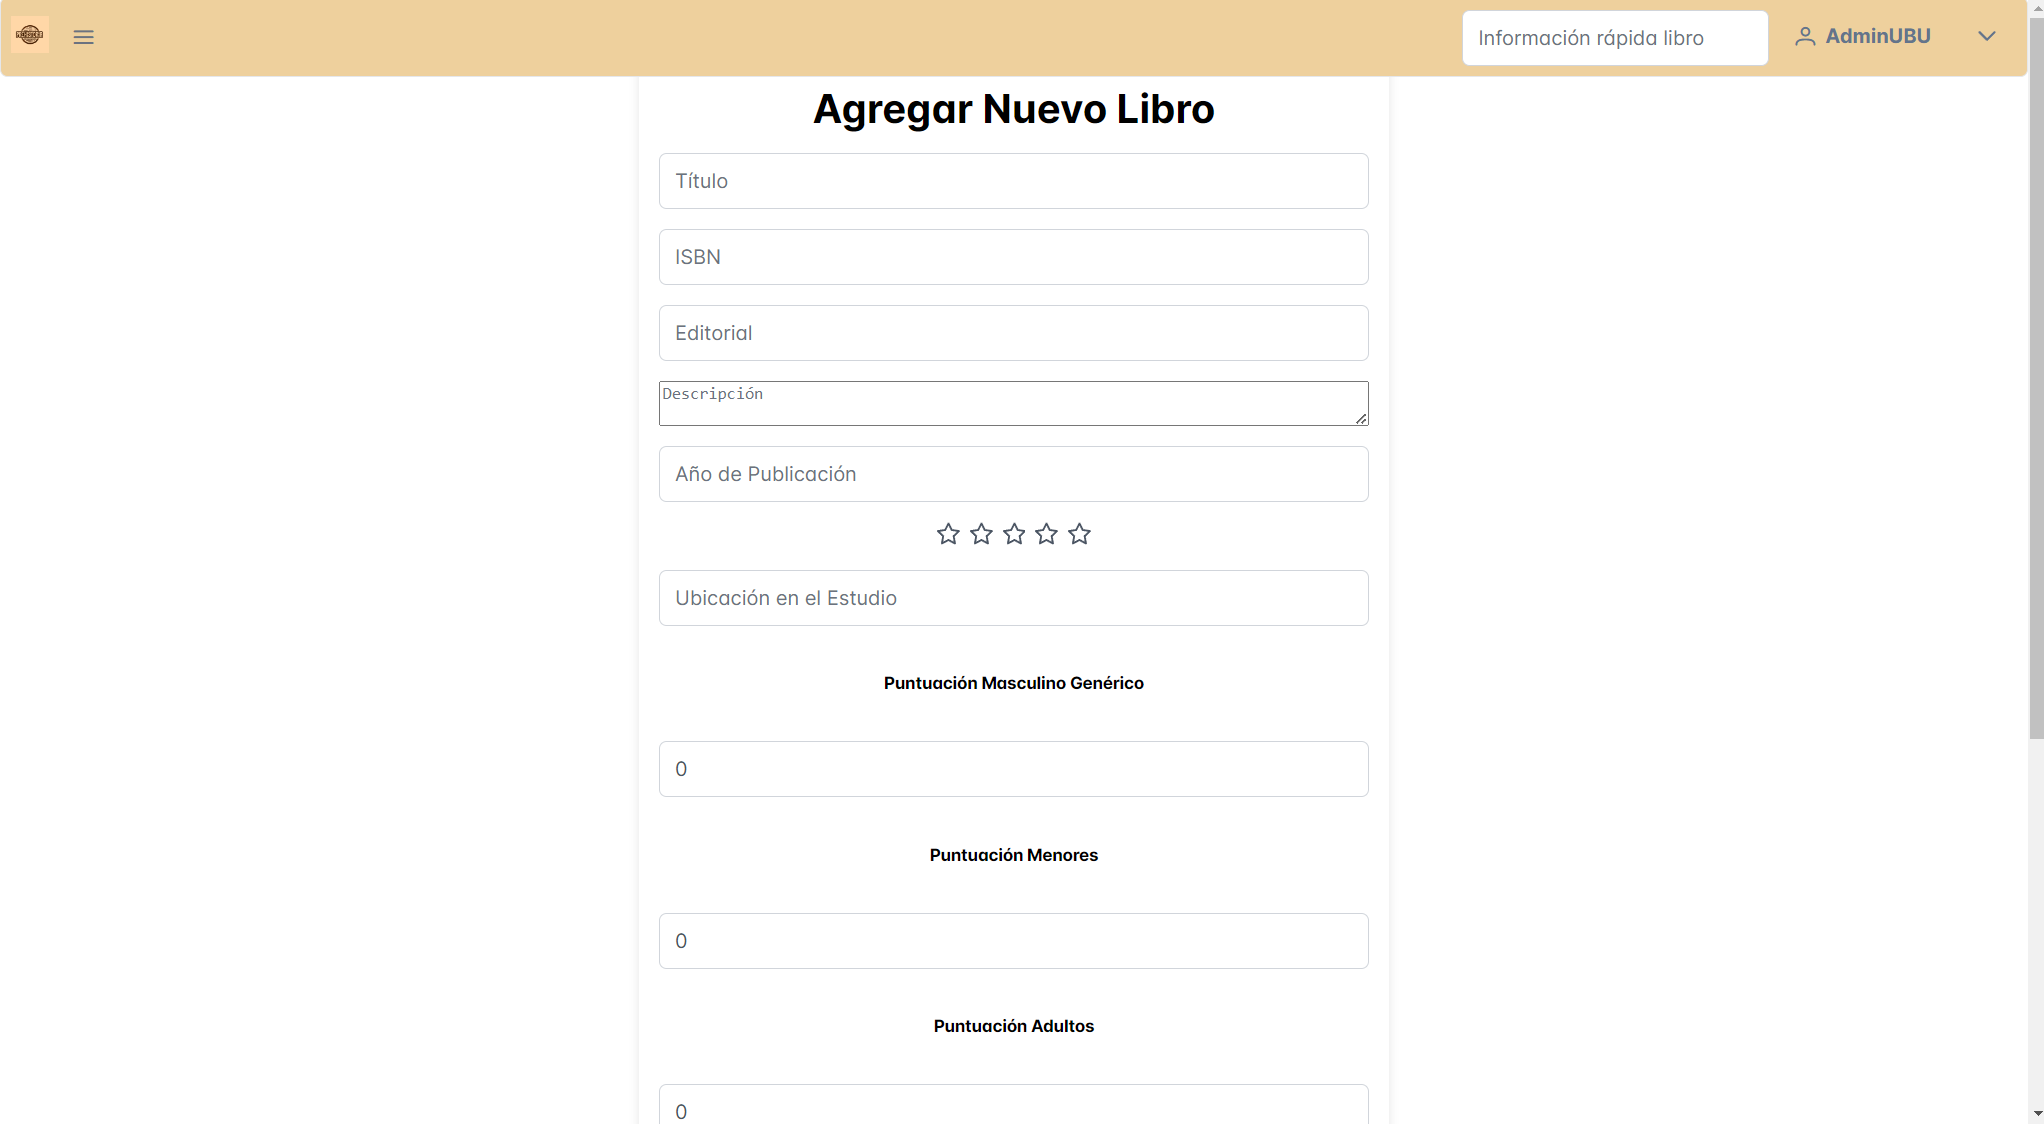
\includegraphics[width=1\linewidth]{Imagenes/ManualAgregar.png}
    \caption{Agregar libro}
    \label{Agregar libro}
\end{figure}

\subsubsection{Agregar un libro automáticamente}
Esta segunda opción ahorra al equipo de administradores el tiempo de encontrar todos los datos utilizando web scraping y la cantidad de datos a rellenar es mucho menor.
Los pasos son los siguientes:

\begin{itemize}
    \item Acceder al panel de administración desde el menú superior.
    \item Desplegar el menú lateral ubicado en el menú de administración y seleccionamos 'agregar libro automáticamente'.
    \item La aplicación muestra una modal donde enviar un título o un ISBN.
    \begin{figure}[h]
        \centering
        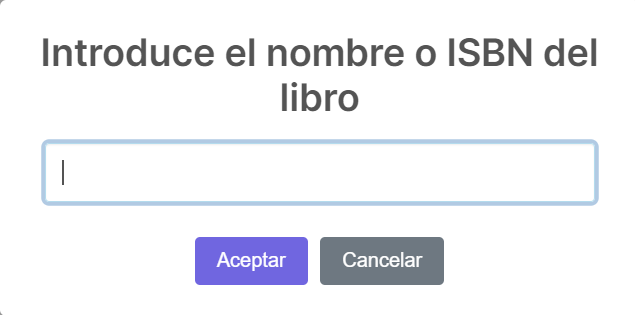
\includegraphics[width=0.5\linewidth]{Imagenes/ManualModalAgregarAuto.png}
        \caption{Modal para agregar automáticamente}
        \label{Modal para agregar automáticamente}
    \end{figure}
    \FloatBarrier
    \item Al enviar esa solicitud aparece una pantalla de carga mientras se buscan posibles libros.
    \item Al terminar la carga aparecerá la información más parecida a la petición realizada en base a 3 fuentes. Abajo del todo aparecerá un botón para ir a agregar un libro manualmente, un botón por cada una de las fuentes para escoger la información de la misma, o un apartado que permite combinar la información de las tres fuentes.
    \begin{figure}[h]
        \centering
        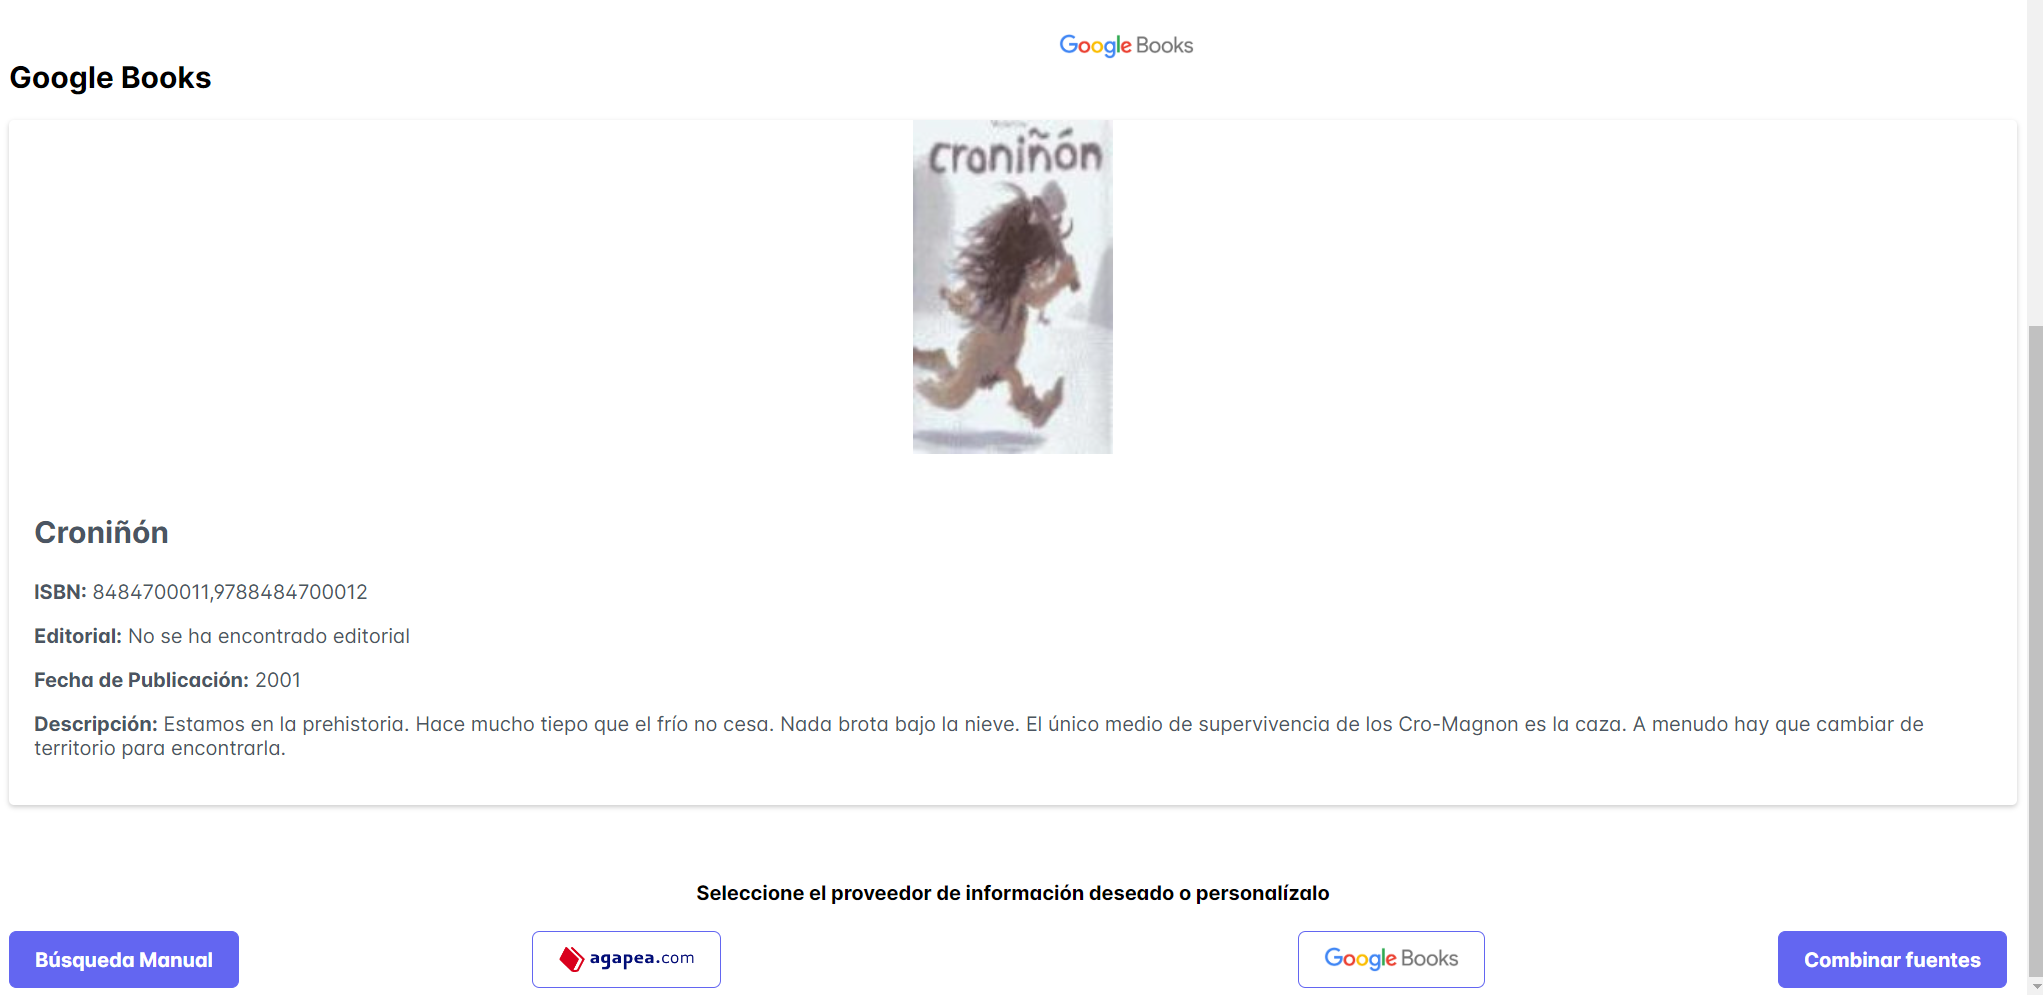
\includegraphics[width=1\linewidth]{Imagenes/ManualSeleccionFuente.png}
        \caption{Selección de fuente de web scraping}
        \label{Selección de fuente de web scraping}
    \end{figure}
    \FloatBarrier

    \item Si se desea agregar un nuevo libro con fuente exclusiva:
    \begin{enumerate}
        \item Se selecciona el botón de esa fuente.
        \item La aplicación se redirigirá al formulario de agregar libro pero con los campos obtenidos autocompletados.
        \item Guardar los cambios.
    \end{enumerate}
    \item Si se desea agregar un nuevo libro con fuentes combinadas:
    \begin{enumerate}
        \item Hacer click en botón de combinar fuentes.
        \item Aparecerá un formulario con los mismos campos que agregar libro pero con desplegables, conteniendo la información de cada fuente, para así seleccionar en cada campo la deseada.
        \item Guardar los cambios.
    \end{enumerate}
\end{itemize}

\begin{figure}[h]
    \centering
    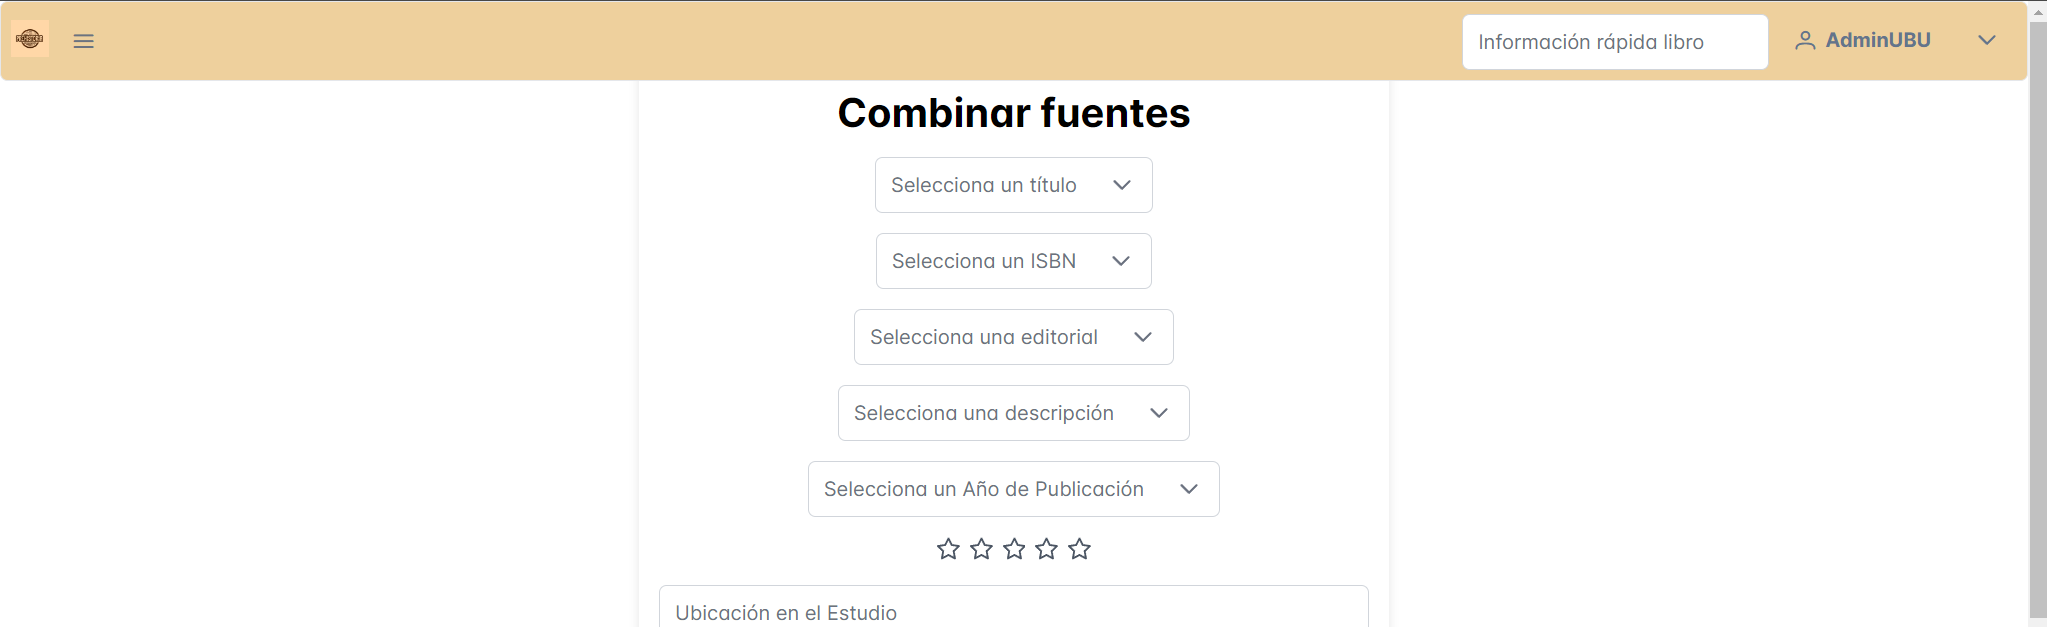
\includegraphics[width=1\linewidth]{Imagenes/ManualCombinar.png}
    \caption{Agregar libro combinando fuentes}
    \label{Agregar libro combinando fuentes}
\end{figure}
\FloatBarrier

\subsection{Gestionar Catálogo}
Además de la herramienta de agregar, el catálogo tiene opciones de editar y eliminar, los pasos para realizar estas operaciones son las siguientes:

\begin{itemize}
    \item Acceder al panel de administración desde el menú superior.
    \item Desplegar el menú lateral ubicado en el menú de administración y seleccionamos 'gestión de catálogo'.
    \item Si se desea editar un libro:
    \begin{enumerate}
        \item Hacer click en el lápiz correspondiente al libro.
        \item Modificar el libro con los campos deseados.
        \item Guardar los cambios.
    \end{enumerate}
    \item Si se desea eliminar un libro:
    \begin{enumerate}
        \item Hacer click en la papelera correspondiente.
        \item Confirmar en la modal la operación.
    \end{enumerate}
\end{itemize}

Finalmente, existe un icono de información en cada libro que redirige a la información del libro seleccionado.
\begin{figure}[h]
    \centering
    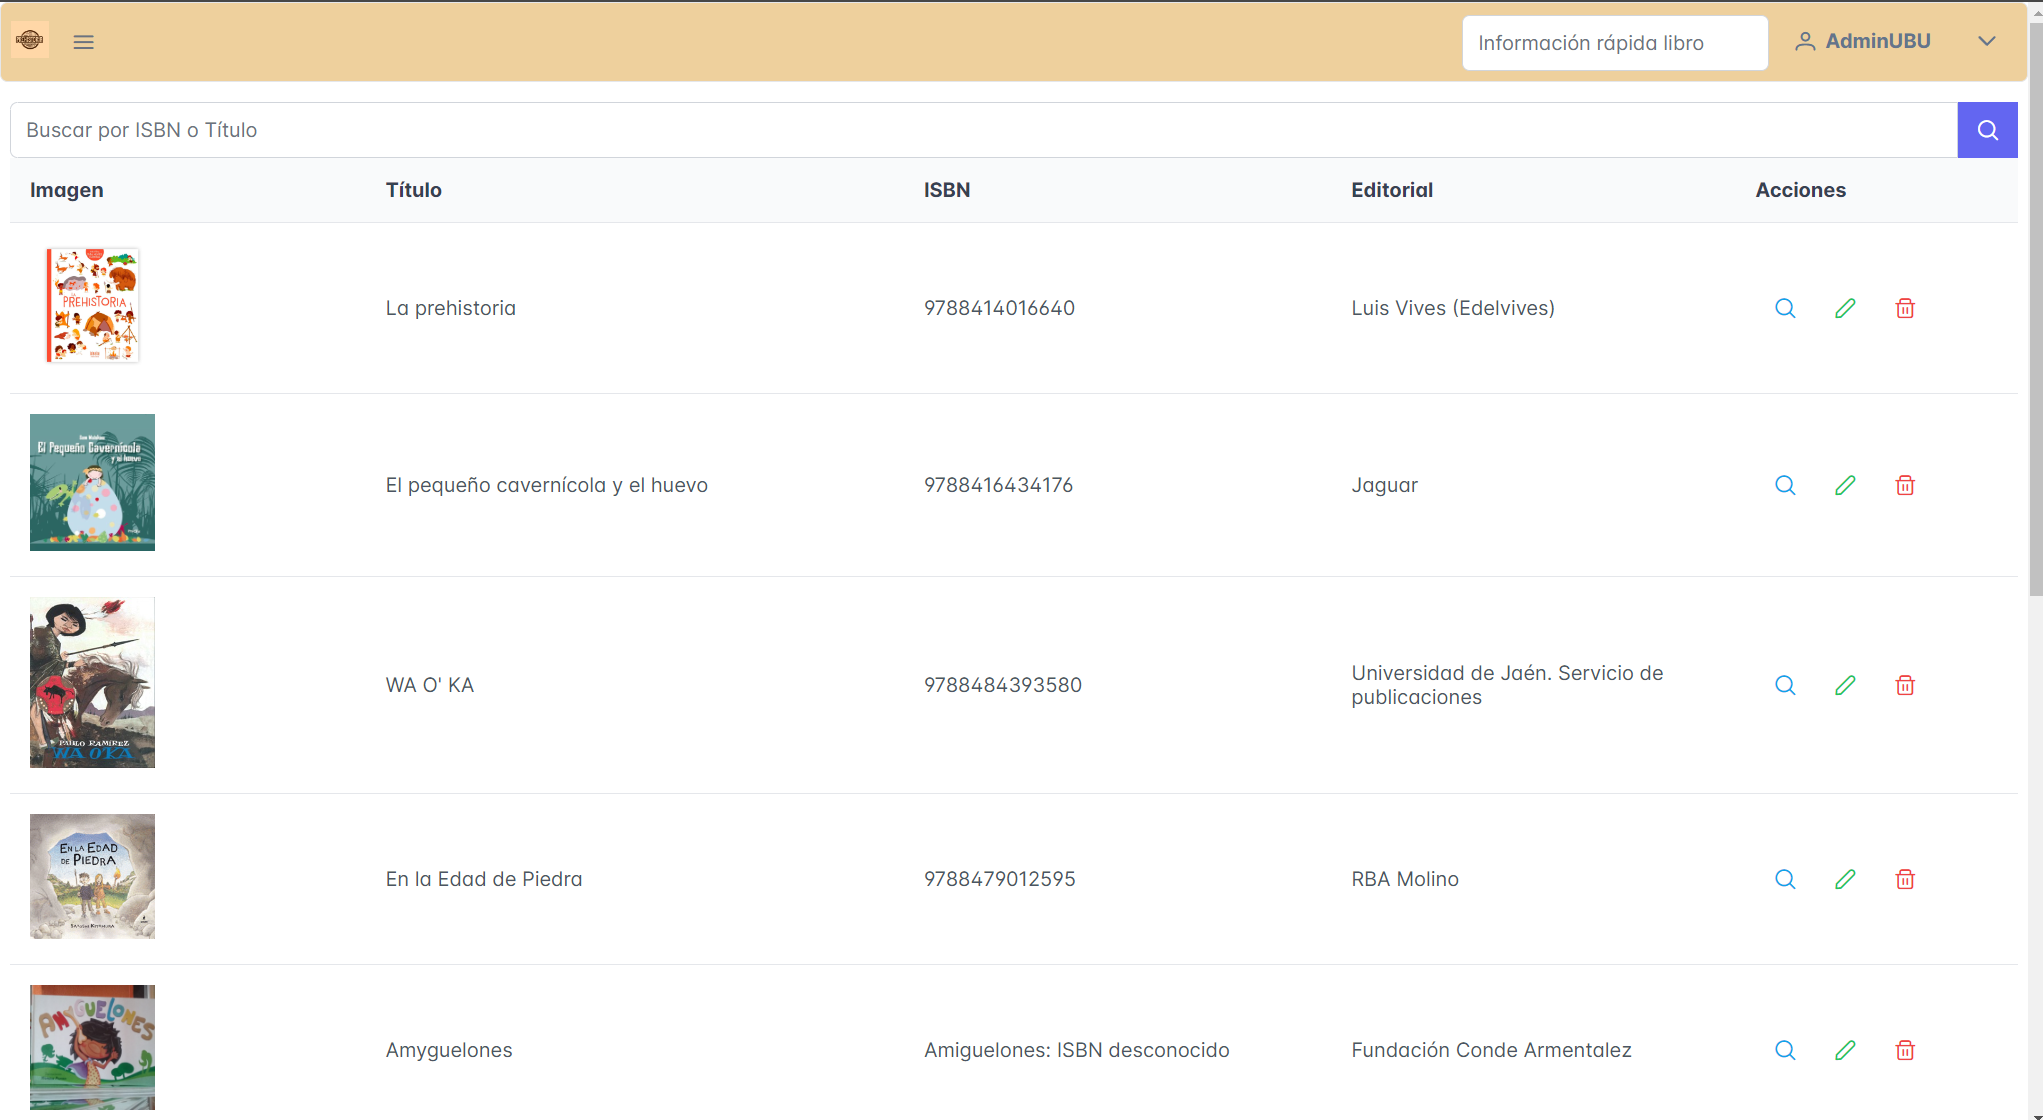
\includegraphics[width=1\linewidth]{Imagenes/ManualGestionCatalogo.png}
    \caption{Pantalla gestión del catálogo}
    \label{Pantalla gestión del catálogo}
\end{figure}
\FloatBarrier

\subsection{Importar y exportar el catálogo}
Para facilitar las labores de agregar libros ya analizados y poder mantener copias de seguridad, se ha facilitado una característica de la aplicación web que permite realizar estas operaciones. A continuación se detallan los pasos:

\begin{itemize}
    \item Acceder al panel de administración desde el menú superior.
    \item Desplegar el menú lateral ubicado en el menú de administración y seleccionamos 'importación o exportación'.
    \item Si se desea importar:
    \begin{enumerate}
        \item Se selecciona el archivo a cargar (Tiene que ser xlsx o csv con separador ;).
    \end{enumerate}
    \item Si se desea exportar:
    \begin{enumerate}
        \item Seleccionar en la modal la extensión con la que se desea exportar.
    \end{enumerate}
\end{itemize}

Es importante mencionar que los archivos a cargar han de incluir todas las siguientes columnas (separadas por ; ):
\begin{itemize}
    \item ID
    \item Título
    \item ISBN
    \item Editorial
    \item Descripción
    \item Año de publicación
    \item Puntuación
    \item Ubicación del estudio
    \item URL de la imagen
    \item Visitas mensuales
    \item Visitas totales
    \item Mes de creación
    \item Año de creación
    \item Puntuación Lenguaje genérico
    \item Puntuación Menores
    \item Puntuación Adultos
    \item Puntuación Ubicación
    \item Puntuación Actividades
\end{itemize}

Es importante destacar que para que la importación/exportación funcione correctamente \textbf{el ISBN debe de ir entre comillas dobles y el campo ID debe de ser único}.

\subsection{Gestión de actividades}
En este apartado se permite al equipo de administración modificar según necesiten las actividades mostradas al generar una valoración.
Los pasos son los siguientes:

\begin{itemize}
    \item Acceder al panel de administración desde el menú superior.
    \item Desplegar el menú lateral disponible en el menú de administración y seleccionar 'gestión de actividades'.
    \item La aplicación muestra las actividades existentes.
    \item Si se desea crear una nueva actividad:
    \begin{enumerate}
        \item Hacer click en el botón de nueva actividad.
        \item Introducir el nombre deseado y las categorías deseadas.
        \item Si se ha creado correctamente, aparecerá una modal el éxito de la operación.
    \end{enumerate}
    \item Si se desea modificar una actividad existente:
    \begin{enumerate}
        \item Hacer click en el lápiz correspondiente a esa actividad.
        \item Introducir el nuevo nombre y las categorías a cambiar.
        \item Si se ha modificado correctamente, aparecerá una modal indicando éxito en la operación.
    \end{enumerate}
    \item Si se desea eliminar un rol:
    \begin{enumerate}
        \item Hacer click en la papelera correspondiente a esa actividad.
    \end{enumerate}
\end{itemize}

\begin{figure}[h]
    \centering
    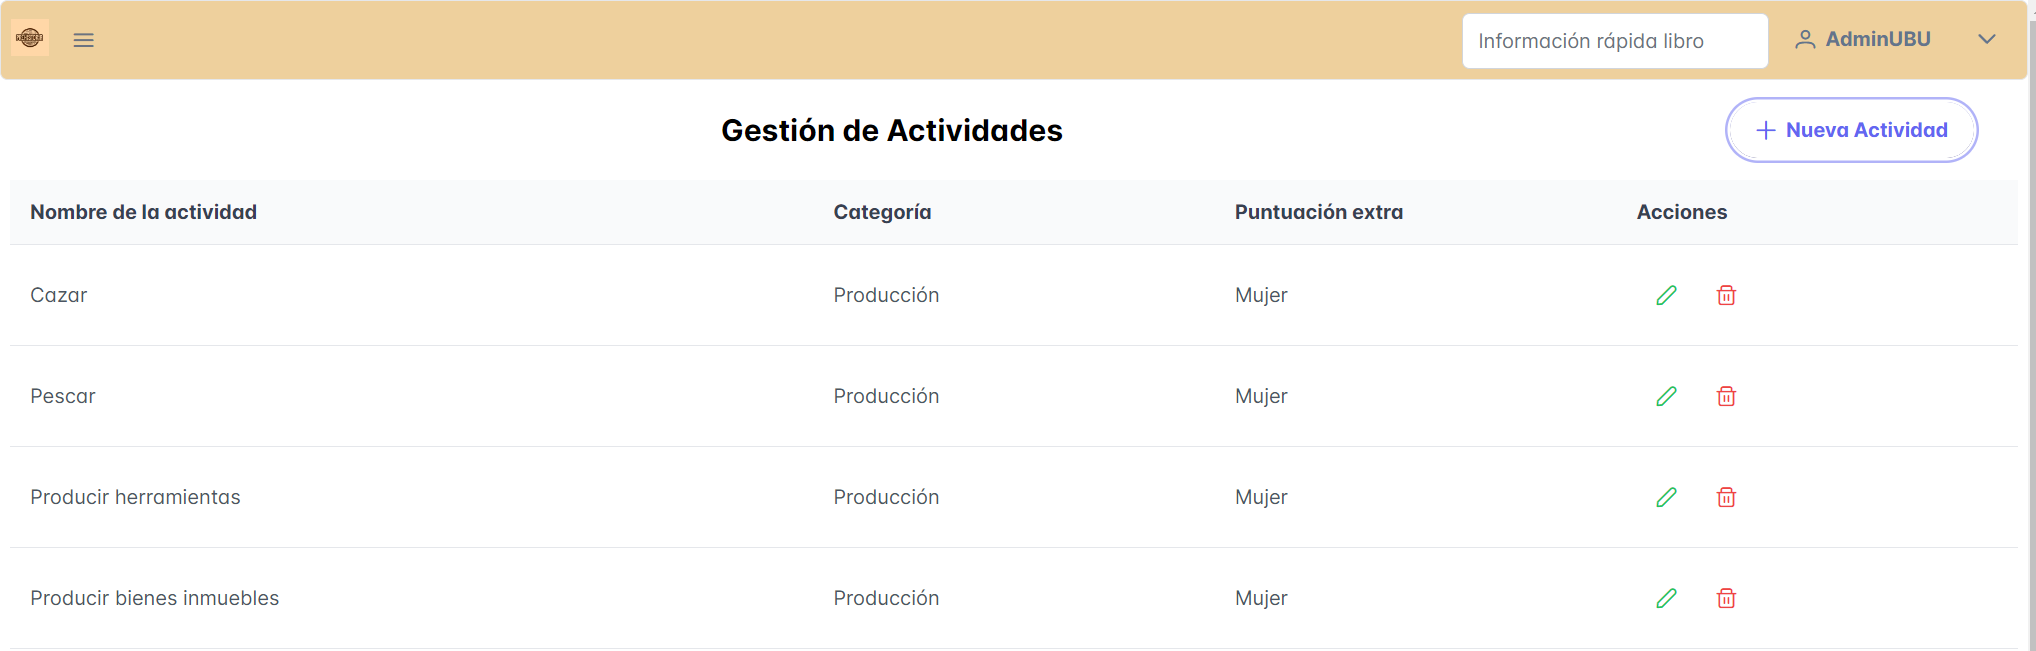
\includegraphics[width=1\linewidth]{Imagenes/ManualActividades.png}
    \caption{Gestión de actividades}
    \label{Gestión de actividades}
\end{figure}
\FloatBarrier

\subsection{Gestionar valoraciones realizadas}
Esta característica de la aplicación permite al equipo de administración observar y eliminar todas las valoraciones que han hecho los usuarios/as.

\begin{itemize}
    \item Acceder al panel de administración desde el menú superior.
    \item Desplegar el menú lateral disponible en el menú de administración y seleccionar 'gestión de valoraciones'.
    \item La aplicación muestra las valoraciones existentes.
    \item Si se desea ver los datos de una valoración existente:
    \begin{enumerate}
        \item Hacer click en el icono de información correspondiente a esa actividad.
        \item Se muestra una modal con toda la información disponible.
    \end{enumerate}
    \item Si se desea eliminar una valoración:
    \begin{enumerate}
        \item Hacer click en la papelera correspondiente a esa valoración.
    \end{enumerate}
    \item Si se desea descargar una valoración:
    \begin{enumerate}
        \item Hacer click en el icono de descargar correspondiente a esa valoración.
        \item Se abrirá una pestaña para ver la dirección de guardado del csv.
    \end{enumerate}
\end{itemize}

\begin{figure}[h]
    \centering
    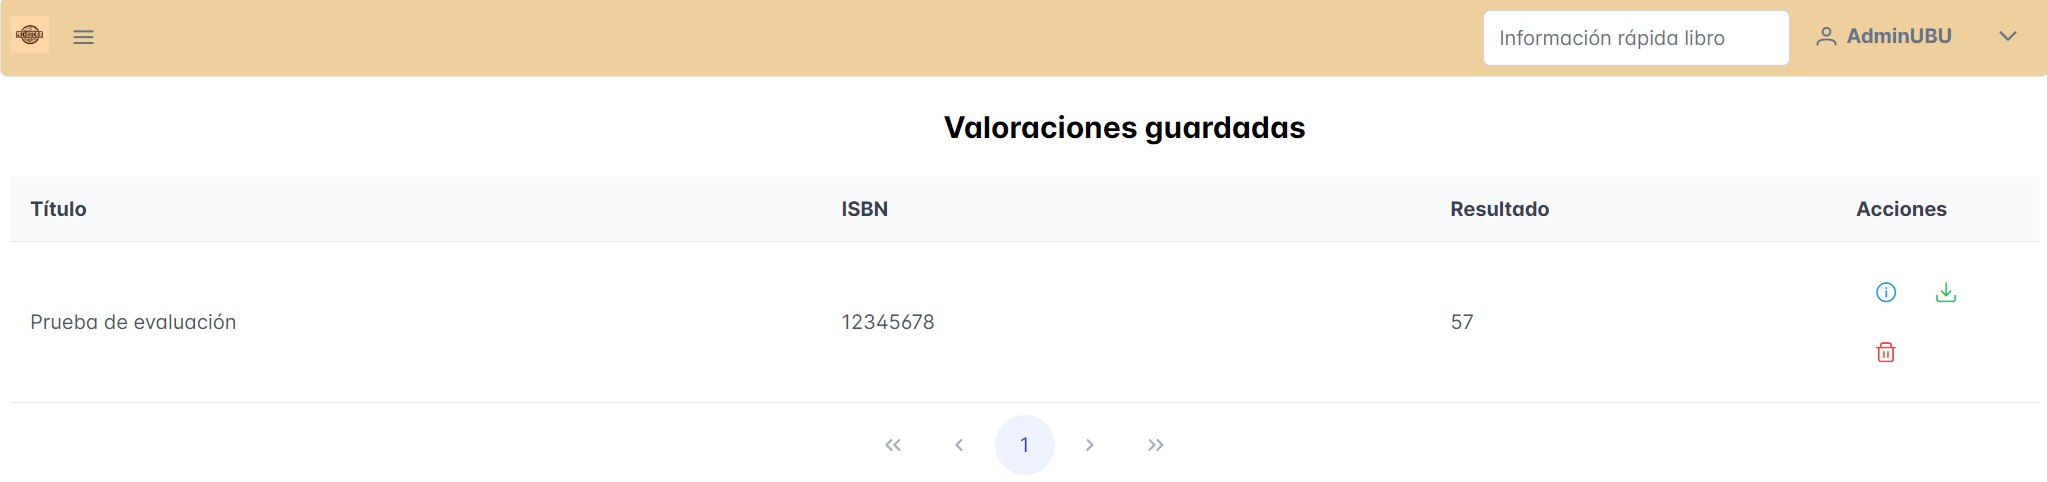
\includegraphics[width=1\linewidth]{Imagenes/ManualValoracionesGuardadas.png}
    \caption{Listado de valoraciones guardadas}
    \label{Listado de valoraciones guardadas}
\end{figure}
\FloatBarrier